% TikZ 复刻。原图：assets/grating-placement.png
% 回退：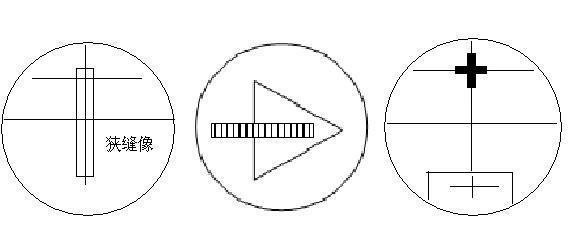
\includegraphics[width=0.70\linewidth]{assets/grating-placement.png}
% 光栅平面垂直平分螺钉 1、2 连线，螺钉 3 位于光栅平面内。
\begin{tikzpicture}[font=\small]
  \def\R{2.05}
  \coordinate (S1) at (180:\R);
  \coordinate (S2) at (0:\R);
  \coordinate (S3) at (270:\R);
  \draw[thick] (0,0) circle (\R);
  \draw[dashed] (S1)--(S2);
  \draw[thin] (0,\R) -- (0,-\R);
  \filldraw[fill=white, thick] (S1) circle (0.15);
  \filldraw[fill=white, thick] (S2) circle (0.15);
  \filldraw[fill=white, thick] (S3) circle (0.15);
  \node[left] at (S1) {$1$};
  \node[right] at (S2) {$2$};
  \node[below] at (S3) {$3$};
  % grating along the perpendicular bisector (vertical diameter),
  % stopped before screw 3
  \filldraw[fill=gray!25, thick] (-0.13,-1.15) rectangle (0.13,1.55);
  \node[right] at (0.55,0.85) {光栅};
  \draw[thin] (0.13,0.70) -- (0.50,0.82);
\end{tikzpicture}
